\documentclass[../Maxima_Workbook.tex]{subfiles}

\begin{document}
	
\chapter{Graphical representation of functions}

\section{Introduction}

There are two different Maxima interfaces for plotting, both being based on \emph{GNUplot}: \emph{plot} and \emph{draw}. Both interfaces are able to deliver 2D and 3D representations. Although they cover the same kind of problems, the two interfaces are substantially different with respect to the structure of their commands, so we treat them separately. \emph{Plot} is the older interface, offering less functionality, but being easier at the same time, so we describe it first.

\lz Both \emph{plot} and \emph{draw} come with additional special functions for use with wxMaxima only. These functions start with the prefix \emph{wx} (e.g. \emph{wxplot2d}, \emph{wxplot3d}). They are the same as the ordinary functions \emph{plot2d} and \emph{plot3d}, with the only difference that they do not open a separate window to display the plot, but instead integrate it into the output of the \emph{.wxm} file or into the \emph{.wxmx} file.

\section{Plot}

\subsection{General}

\subsubsection{Options, (user) standard options, and system standard options}

The user can customize any of the plot functions by setting plot options. This can be done individually for each function call. It is also possible to set \emph{(user) standard options} which then apply to any function call unless they are overwritten by it. Certain individual options cannot be set as standard, see details in the description of plot options.

\lz Certain options are set standard by the system already, e.g. the order of colors in a multiple plot, if no colors are specified by the user. They can be viewed with the following function.

\lzz \hyt{set\_plot\_option}{\tcr{\emph{set\_plot\_option $ ( \glangle option_1,\dots,option_n \grangle ) $}}} \hfill \tcr{[function]}\index{set\_plot\_option}

\hyt{get\_plot\_option}{\tcr{\emph{get\_plot\_option $ (name \, \glangle, index \grangle ) $}}} \hfill \tcr{[function]}\index{get\_plot\_option}

\hyt{remove\_plot\_option}{\tcr{\emph{remove\_plot\_option (name)}}} \hfill \tcr{[function]}\index{remove\_plot\_option}

\lz Setting \emph{(user) standard options} is done with function \emph{set\_plot\_option}. Each option is a list in square brackets, as described below. \emph{set\_plot\_option} returns a list not only of the standard options currently set by the user, but also of all \emph{system standard options}. Giving an empty set of parentheses to this function will only return the currently set (user and system) standard options without adding any to them.

\lz \emph{get\_plot\_option} returns as a list in square brackets the current standard setting of the option \emph{name}. If the second argument \emph{index} is present, only the \emph{index}th element of this list will be returned (the first element is the option name).

\lz \emph{remove\_plot\_option} removes from the list of standard options the option \emph{name}. Note that this function requires exactly one argument; multiple removals are not possible.

\subsubsection{Options for both 2D and 3D plots}\label{Pl1}

All options (this also holds for the options specific to either 2D or 3D as described in sections \ref{Pl2} and \ref{Pl3}) consist of a list (in square brackets) starting with one of the keywords in this section, followed by one or more values. (This layout is comparable to a function name and its arguments.) The options that accept among their possible values \emph{true} or \emph{false}, can also be set to \emph{true} by simply writing their names. For instance, typing \emph{logx} as an option is equivalent to writing \emph{[logx, true]}.

\lzz \hyt{plot-box}{\tcr{\emph{[box, true \gbar $ \, $false]}}} \qquad \tcr{default: \emph{true}} \hfill \tcr{[plot option]}\index{plot!box}

\lz If set to \emph{true}, a bounding box will be drawn around the plot; if set to \emph{false}, no box will be drawn.

\lzz \hyt{plot-color}{\tcr{\emph{[color, $ color_1,\dots,color_n $]}}} \hfill \tcr{[plot option]}\index{plot!color}

\lz In 2d plots this option defines the color (or colors) for the various curves. In plot3d, it defines the colors used for the mesh lines of the surfaces, when no palette is being used. If there are more curves or surfaces than colors, the colors will be repeated in sequence. The valid colors are red, green, blue, magenta, cyan, yellow, orange, violet, brown, gray, black, white, or a string starting with the character \# and followed by six hexadecimal digits: two for the red component, two for green component and two for the blue component. If the name of a given color is unknown color, black will be used instead.

\lzz \hyt{plot-legend}{\tcr{\emph{[legend, false \gbar $ \, string_1,\dots,string_n$]}}} \hfill \tcr{[plot option]}\index{plot!legend}

\lz Specifies the labels for the plots when various plots are shown. If there are more
plots than the number of labels given, they will be repeated. If given the value \emph{false}, no legends will be shown. By default, the names of the expressions or functions will be used, or the words $ discrete_1,\dots,discrete_n $ for discrete sets of points.

\lzz \hyt{plot-logx}{\tcr{\emph{[logx, true \gbar $ $ false]}}} \qquad \tcr{default: \emph{false}} \hfill \tcr{[plot option]}\index{plot!logx}

\hyt{plot-logy}{\tcr{\emph{[logy, true \gbar $ $ false]}}} \qquad \tcr{default: \emph{false}} \hfill \tcr{[plot option]}\index{plot!logy}

\lz Makes the horizontal or vertical axes to be scaled logarithmically.

\lzz \hyt{plot-format}{\tcr{\emph{[plot\_format, format]}}} \qquad \tcr{default: \emph{gnuplot \gbar $ $ gnuplot\_pipes}} \hfill \tcr{[plot option]}\index{plot!plot\_format}

\lz Specifies the format for the plot. In Windows the default is \emph{gnuplot}, in all other systems it is \emph{gnuplot\_pipes}. The formats \emph{xmaxima} or \emph{openmath} will cause the plot to be displayed in an xMaxima window.

\lzz \hyt{plot-realpart}{\tcr{\emph{[plot\_realpart, true \gbar $ $ false]}}} \qquad \tcr{default: \emph{false}} \hfill \tcr{[plot option]}\index{plot!plot\_realpart}

\lz If set to \emph{true}, the functions to be plotted will be considered as complex functions whose real part should be plotted; this is equivalent to plotting realpart(function). If set to \emph{false}, nothing will be plotted when the function does not give a purely real value. For instance, when x is negative, log(x) gives a complex value, with the real value equal to log(abs(x)); if \emph{plot\_realpart} were true, log(-5) would be plotted as log(5), while nothing would be plotted if \emph{plot\_realpart} were \emph{false}.

\lz \begin{lstlisting}
<@\tcr{(\%i1)}@   plot2d(realpart(log(x)),[x,-2,2],[y,-4,2]);
<@\tcr{(\%i2)}@   plot2d(log(x),[x,-2,2],[y,-4,2],plot_realpart);
\end{lstlisting}
\vspace{-2mm} 

\lz Both plots will return exactly the same graph.

\begin{SCfigure}[0.33][h]
	\centering
	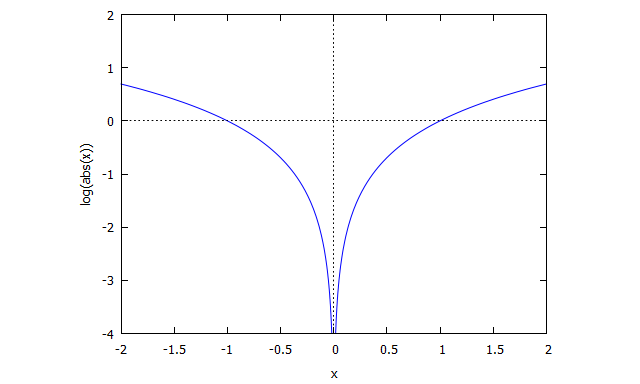
\includegraphics[width=0.75\textwidth]{Pl_plot_realpart.png}
	\caption{Plotting the real part of the complex logarithm.}
	\label{Pl-Fig5}
\end{SCfigure}

\lzz \hyt{plot-same-xy}{\tcr{\emph{[same\_xy, true \gbar $ $ false]}}} \qquad \tcr{default: \emph{false}} \hfill \tcr{[plot option]}\index{plot!same\_xy}

\lz If \emph{true}, displays the graph with the same scale for both x and y axes. For a 2D plot, see also \hyl{plot-yx-ratio}{yx\_ratio}.

\lzz \hyt{plot-xlabel}{\tcr{\emph{[xlabel, string]}}} \hfill \tcr{[plot option]}\index{plot!xlabel}

\hyt{plot-ylabel}{\tcr{\emph{[ylabel, string]}}} \hfill \tcr{[plot option]}\index{plot!ylabel}

\hyt{plot-zlabel}{\tcr{\emph{[zlabel, string]}}} \hfill \tcr{[plot option]}\index{plot!zlabel}

\lz \emph{xlabel} and \emph{ylabel} specify the string that will label the first/second axis; if this option is not used, that label
will be the name of the independent variable / "y", when plotting functions with \emph{plot2d} or \emph{implicit\_plot}, or the name of the first/second variable, when plotting surfaces with \emph{plot3d} or contours with \emph{contour\_plot}, or the first/second expression in the case of a parametric plot.

\lz \emph{zlabel} specifies the string that will label the third axis, when using \emph{plot3d}. If this option is not used, that label will be “z”, when plotting surfaces, or the third expression in the case of a parametric plot. It will be ignored by \emph{plot2d} and \emph{implicit\_plot}.

\lz These options cannot be used with \emph{set\_plot\_option}.

\subsubsection{Zooming the plot}

mails Robert and Laurent, 12.12.2018

\subsection{2D}

There are 5 basic types of 2D plot: explicit plot, parametric plot, discrete plot, implicit plot, and contour plot. The first three are implemented in function \emph{plot2d}, the last two in separate functions.

\subsubsection{plot2d}

\lz \hyt{plot2d}{\tcr{\emph{plot2d ($ \gpal \, plot \, \gbar \, [ plot_1,\dots,plot_n ] \gpar  \glangle, x\_range \grangle \glangle, y\_range \grangle \glangle, options \grangle $)}}} \hfill \tcr{[function]}\index{plot2d}

\hyt{wxplot2d}{\tcr{\emph{wxplot2d(...)}}} \hfill \tcr{[function]}\index{wxplot2d}

\lz These functions plot a two-dimensional graph of \\
- an expression giving the y-coordinate as a function of one variable being the x-coordinate (explicit plot), \\
- two expressions, one for the x- and one for the y-coordinate, as being functions of a single common parameter (parametric plot), or \\
- a number of discrete points in the xy-plane (discrete plot). 

\lz Each type can be used in single or multiple form, and different types can be combined to one representation.

\lzz \tcr{\emph{$ plot \gbar [ \, plot_1,\dots,plot_n \, $]}}

\lz A single plot is given as the first argument to \emph{plot2d} while a multiple plot is given as a list (of plots) being the first argument. Each of the plots is either an expression (for an explicit plot), a parametric plot, or a discrete plot.

\paragraph{Explicit plot} \mbox{}

\lz A single 2D explicit plot displays the graph of an expression as a function of one variable. While the independent variable determines the x-coordinate of a plot point, the function value determines its y-coordinate. A multiple explicit plot displays multiple such graphs. An explicit functional expression in terms of the independent variable is given for each individual plot. The independent variable has to be the same for all plots of a multiple explicit plot.

\lzz \tcr{\emph{x\_range}} is of the form: \tcr{\emph{[x\_name, min, max]}}. 

\lz This is mandatory for explicit plots and specifies the name of the independent variable of the expression(s) to be plotted, and the range of its domain to be displayed on the horizontal axis. In case of a multiple explicit plot, the same \emph{x\_range} is used for all expressions. Individual plotting ranges are not possible (in contrast to \emph{plot3d}). Hence, it is not possible to plot a piecewise defined function. In a combination of explicit and parametric plots, the name of the independent variable has to be \emph{x}.

\lzz \tcr{\emph{y\_range}} is of the form: \tcr{\emph{[y, min, max]}}. 

\lz This is optional and specifies the range of the codomain to be displayed on the vertical axis. If this option is used, the plot will show this exact vertical range, independently of the values reached by the plot. Everything outside of the given range will be clipped off. If the vertical range is not specified, it will be set according to the minimum and maximum values of the second coordinate reached by the plot. For \emph{y\_range} the name is always \emph{y}. So it is wise not to use \emph{y} as the name of the independent variable. 

\lzz The complete syntax for an explicit plot is

\lz \hyt{plot2d}{\tcr{\emph{plot2d ($ \gpal \, expr \, \gbar \, [ expr_1,\dots,expr_n ] \gpar  \glangle, x\_range \grangle \glangle, y\_range \grangle \glangle, options \grangle $)}}}

\lz Options are described in sections \ref{Pl1} and \ref{Pl2}. In case of a multiple plot, different colors will be used automatically for the different expressions and a legend will be created. Options present in case of a multiple plot apply to all plots; it is not possible to set options individually.

\lz Note that the separate plot window (not when integrated into the wxMaxima file with wxplot2d) can be scrolled both horizontally and vertically to see beyond the selected ranges. The plot can be exported, e.g. as a \emph{.png} file, directly from the separate plot window.

\lz \begin{lstlisting}
<@\tcr{(\%i1)}@   plot2d([%e^x, %e^(-x), log(x), 1/x, sqrt(x)],[x,-3,5],[y,-10,10]);
\end{lstlisting}
\vspace{-2mm} 

\begin{SCfigure}[0.33][h]
	\centering
	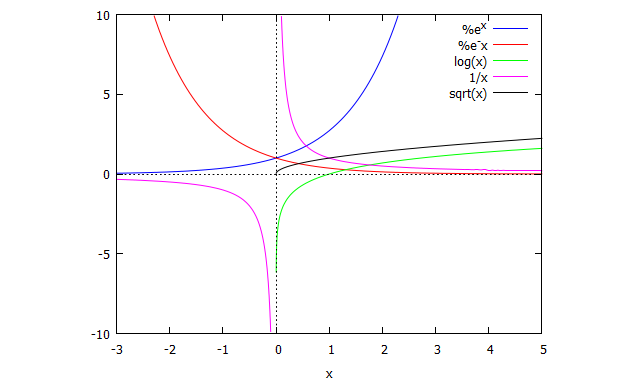
\includegraphics[width=0.75\textwidth]{Pl_explicit_plot2d.png}
	\caption{Multiple 2D explicit plot.}
	\label{Pl-Fig1}
\end{SCfigure}

\paragraph{Parametric plot} \mbox{}

\lz A single 2D parametric plot displays a graph generated in parallel by two different expressions, one for the x- and one for the y-coordinate, as being functions of a common single parameter. The name of the parameter always has to be t. A multiple parametric plot displays multiple such graphs. The complete syntax for a single parametric plot is

\lz \tcr{\emph{plot3d ([parametric, $ expr_x, expr_y $, [t, min, max]] $ \glangle, options \grangle $)}}.

\lz This creates a curve in in the two-dimensional space $ expr_x \times expr_y $ in terms of the parameter t ranging from \emph{min} to \emph{max}. 

\lz Neither \emph{x\_range} nor \emph{y\_range} have to be present. When they are, they will specify the ranges to be displayed in the graph for the horizontal and the vertical axis. When they are not present, ranges will be set according to the minimum and maximum values of the coordinates reached by the plot points.

\lz \begin{lstlisting}
<@\tcr{(\%i1)}@   plot2d([[parametric, sin(t), cos(t),[t,0,2*%pi]],[parametric, sin(t), cos(t)/2,[t,0,2*%pi]]],same_xy);
\end{lstlisting}
\vspace{-2mm} 

\begin{SCfigure}[0.33][h]
	\centering
	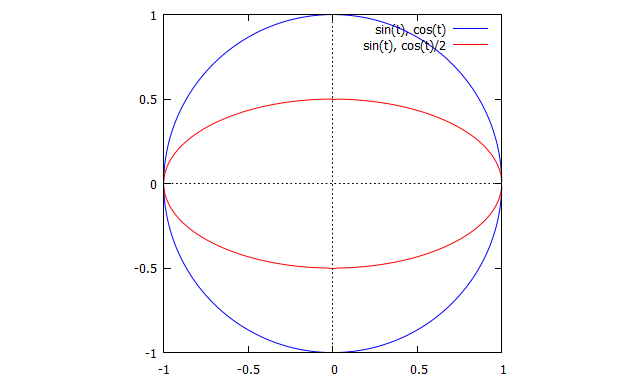
\includegraphics[width=0.75\textwidth]{Pl_parametric_plot2d.png}
	\caption{Multiple 2D parametric plot.}
	\label{Pl-Fig2}
\end{SCfigure}

\paragraph{Discrete plot} \mbox{}

\lz A single 2D discrete plot displays a graph consisting of a number of discrete points specified explicitly by their x- and y-coordinates. A multiple discrete plot displays multiple such graphs. The syntax for a single discrete plot is

\lz \tcr{\emph{ $ [discrete, xlist, ylist] \, \gbar \, [discrete, [[ x_1,y_1],\dots,[x_n,y_n]]$}}

\lz This creates a plot of n discrete points, where \emph{xlist} and \emph{ylist} are lists in square brackets of n elements each, containing in sequence the x- resp. y-coordinates of the points to be plotted. So the coordinates of the points can be enterd either separately for x- and y- valuse, or point by point. If no option \emph{styles} is present, by default \emph{[style, lines]} is assumed, that is, the discrete points are linked by line segments, see section \ref{Pl2}.

\lz \begin{lstlisting}
<@\tcr{(\%i1)}@   plot2d([[discrete, makelist(i,i,1,10),makelist(sqrt(i),i,1,10],[discrete, makelist(i,i,0,10),makelist(sqrt(i)+sin(i),i,0,10)]],[style,points],[point_type,plus]);
\end{lstlisting}
\vspace{-2mm} 

\begin{SCfigure}[0.33][h]
	\centering
	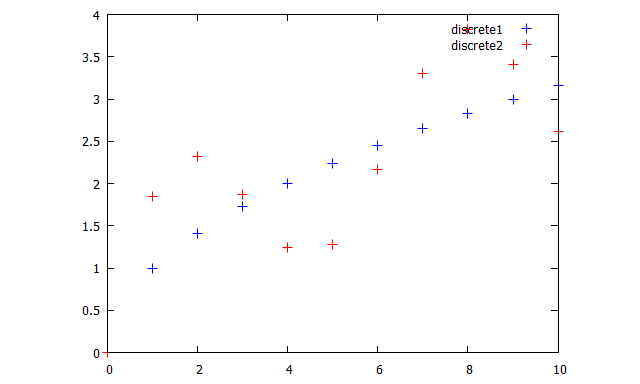
\includegraphics[width=0.75\textwidth]{Pl_discrete_plot2d.png}
	\caption{Multiple discrete plot2d. The x- and y-coordinates of the points are generated by function \emph{makelist}.}
	\label{Pl-Fig6}
\end{SCfigure}

For more examples see the examples to the function \emph{rk} implementing the Runge-Kutta method for numerically solving a first order ODE.

\lz Combining a discrete with an explicit plot, e.g., it is possible to represent the discrete data of an experiment together with a theoretically assumed continuous function to interpret them.

\subsubsection{Implicit plot}

A single 2D implicit plot displays the graph of a function given implicitly by an equation containing both the independent (x-coordinate) and the dependent (y-coordinate) variable. This equation does not have to be in explicit form.

\lz \hyt{implicit\_plot}{\tcr{\emph{implicit\_plot ($ \gpal eq \, \gbar \, [eq_1,\dots,eq_n \, ] \gpar $, x\_range, y\_range $ \glangle, options \grangle $)}}} \hfill \tcr{[function]}\index{implicit\_plot}

\hyt{wximplicit\_plot}{\tcr{\emph{wximplicit\_plot(...)}}} \hfill \tcr{[function]}\index{wximplicit\_plot}

\lz In the first case this plots a single function defined implicitly by equation \emph{equ}. The syntax is similar to \emph{plot2d}. The domain is defined by \emph{x\_range} and \emph{y\_range} which are both mandatory. Both variable names can be selected freely. Multiple implicit plots can be combined to a graph by giving a list of equations [$ eq_1,\dots, eq_n $], one for each plot. Before it can be used this function has to be loaded.

\lz \begin{lstlisting}
<@\tcr{(\%i1)}@   load(implicit_plot);
<@\tcr{(\%i1)}@   implicit_plot([x^2+y^2=1, (x/2)^2+y^2=1/4], [x,-1,1], [y,-1,1], same_xy);
\end{lstlisting}
\vspace{-2mm} 

\begin{SCfigure}[0.33][h]
	\centering
	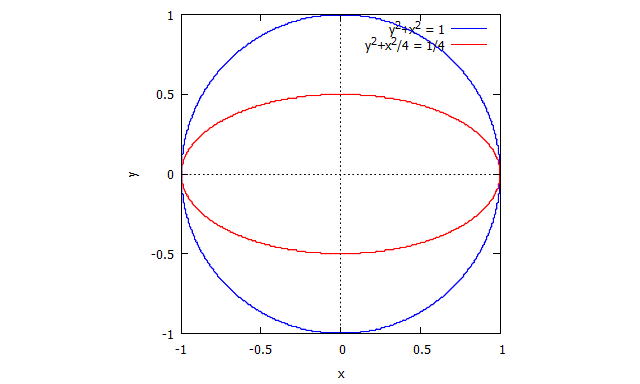
\includegraphics[width=0.75\textwidth]{Pl_implicit_plot.png}
	\caption{Multiple implicit plot. The resulting curves are the same as in the multiple parametric plot of Fig. \ref{Pl-Fig2}.}
	\label{Pl-Fig3}
\end{SCfigure}

\subsubsection{Contour plot}

A 2D contour plot displays contours (curves of equal value) of a scalar-valued function of two arguments over a 2D region defined by the domains of these two arguments. Such a function can be considered a scalar field.

\lz \hyt{contour\_plot}{\tcr{\emph{contour\_plot (expr, x\_range, y\_range $ \glangle, [opt_1],\dots,[opt_n] \grangle $)}}} \hfill \tcr{[function]}\index{contour\_plot}

\hyt{wxcontour\_plot}{\tcr{\emph{wxcontour\_plot(...)}}} \hfill \tcr{[function]}\index{wxcontour\_plot}

\lz This plots several curves of equal value of \emph{expr} over the region defined by \emph{x\_range} and \emph{y\_range}. The names of the x- and y-coordinates can be selected freely. \emph{contour\_plot} accepts only options which can be used for \emph{plot3d}. Each one of them has to be present as a list, i.e. the abbreviation of giving only the name of an option to indicate its value as true, is not allowed. Some of these options, e.g. \emph{same\_xy}, will cause the 2D plot to be displayed in a 3D representation. 

\lz \begin{lstlisting}
<@\tcr{(\%i1)}@   contour_plot(x/y,[x,-2,2],[y,-2,2]);
\end{lstlisting}
\vspace{-2mm} 

\begin{SCfigure}[0.33][h]
	\centering
	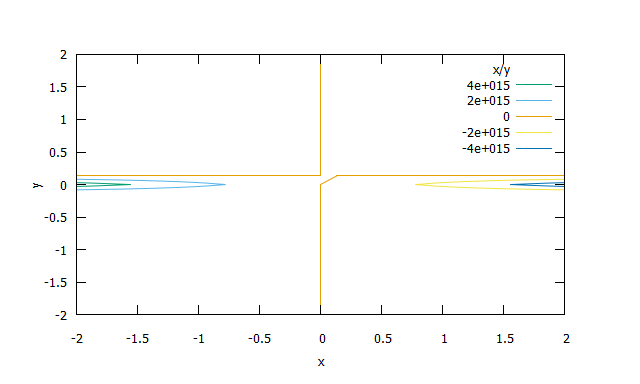
\includegraphics[width=0.75\textwidth]{Pl_contour_plot.png}
	\caption{Contour plot.}
	\label{Pl-Fig4}
\end{SCfigure}

\subsubsection{Options for 2D}\label{Pl2}

\lz \hyt{plot-axes}{\tcr{\emph{[$axes, \gpal value \, \gbar \, false \gpar$]}}} \qquad \tcr{default: \emph{true}} \hfill \tcr{[plot option]}\index{plot!axes}

\lz \emph{value} can be either \emph{true}, \emph{false}, \emph{x}, \emph{y} or \emph{solid}. If \emph{false}, no axes are shown; if \emph{x} or \emph{y}, only the \emph{x} or \emph{y} axis will be shown; if \emph{true}, both axes will be shown. \emph{solid} will show the two axes with a solid line, rather than the default broken line.

\lzz \hyt{plot-point-type}{\tcr{\emph{[point\_type, $ type_1,\dots,type_n $]}}} \hfill \tcr{[plot option]}\index{plot!point\_type}

\lz Each set of points to be plotted with the style \emph{points} or \emph{linespoints} will be represented with objects taken from this list, in sequential order. If there are more sets of points than objects in this list, they will be repeated sequentially. The possible objects that can be used are: bullet, circle, plus, times, asterisk, box, square, triangle, delta, wedge, nabla, diamond, lozenge.

\lzz \hyt{plot-style}{\tcr{\emph{[style, $ style_1 $ \gbar [$ \, style_1 $]$ ,\dots,style_n, $ \gbar [$ \, style_n $]]}}} \hfill \tcr{[plot option]}\index{plot!style}

\lz Describes the style(s) of the plot(s). If there are more plots than styles present, the styles will be repeated sequentially. Each style is either given by its name only, or as a list with additional arguments. In the first case, standard values are assumed for the style. In the second case, the first element of the list is the name of the style, followed by the arguments.

\lz Each style can be either \emph{lines} for line segments, \emph{points} for isolated points, \emph{linespoints} for segments and points, or \emph{dots} for small isolated dots. Gnuplot accepts also an \emph{impulses} style. If enclosed in a list, \emph{lines} accepts one or two arguments: the width of the line and an integer that identifies a color. The default color codes are: 1: blue, 2: red, 3: magenta, 4: orange, 5: brown, 6: lime and 7: aqua. If Gnuplot is used with a terminal different than X11, those colors might be different. \emph{points} accepts one to three arguments; the first one is the radius of the points, the second one is an integer that selects the color, using the same code used for lines and the third one is currently used only by Gnuplot and it corresponds to several objects instead of points. The default types of objects are: 1: filled circles, 2: open circles, 3: plus signs, 4: x, 5: *, 6: filled squares, 7: open squares, 8: filled triangles, 9: open triangles, 10: filled inverted triangles, 11: open inverted triangles, 12: filled lozenges and 13: open lozenges. Note that point types can be specified with option \emph{point\_type}, see above. \emph{linespoints} accepts up to four arguments: line width, points radius, color and type of object to replace the points.

\lzz \hyt{plot-yx-ratio}{\tcr{\emph{[yx\_ratio, r]}}} \hfill \tcr{[plot option]}\index{plot!yx\_ratio}

\lz \emph{r} defines the ratio between the vertical and the horizontal sides of the rectangle used to make the plot. See also \hyl{plot-same-xy}{same\_xy}.

\subsection{3D}

In 3D only two basic types of plot are possible: explicit plot and parametric plot. They are both implemented in function \emph{plot3d}. Implicit 3D plots are possible only with \emph{draw3d}.

\subsubsection{plot3d}

\lz \hyt{plot3d}{\tcr{\emph{plot3d (plot $ \glangle, options \grangle $)}}} \hfill \tcr{[function]}\index{plot3d}

\hyt{wxplot3d}{\tcr{\emph{wxplot3d(...)}}} \hfill \tcr{[function]}\index{wxplot3d}

\lz These functions plot a three-dimensional graph of \\
- an expression giving the z-coordinate as a function of two variables being the x- and the y-coordinates (explicit plot),
- three expressions, one for each of the x-, y-, and z-coordinates, as being functions of two common parameters (parametric plot). 

\lz Multiple explicit plots can be combined to one representation. In contrast to plot2d, however, only single parametric plots can be displayed, and the combination of explicit and parametric plots is not possible, either.

\paragraph{Explicit plot} \mbox{}

\lz A single 3D explicit plot displays the graph of an expression giving the z-coordinate as a function of two variables being the x- and y-coordinates. A multiple explicit plot displays multiple such graphs. In this case, an explicit functional expression in terms of the independent variables is given for each individual plot.

\lz For a single plot, the explicit functional expression is given as the first argument to \emph{plot3d}. In this case, \emph{x\_range} and \emph{y\_range} have to be the second and third argument, possibly followed by options. The complete syntax for a single plot is

\lz \tcr{\emph{plot3d (expr, x\_range,  y\_range $ \glangle, options \grangle $)}}.

\lz A multiple explicit plot can have two different forms, depending on whether the individual plots share the same x\_range and y\_range or not. In both cases, and in contrast to plot2d, x\_range and y\_range form part of the list of plots. The syntax for a multiple explicit plot using the same x\_range and y\_range is

\lz \tcr{\emph{plot3d ([$expr_1,\dots,expr_n, x\_range,  y\_range $] $ \glangle, options \grangle $)}}.

\lz The syntax for a multiple plot using a different x\_range and y\_range for each individual plot is

\lz \tcr{\emph{plot3d ([[$expr_1,x\_range_1,  y\_range_1 $],$\dots $,[$expr_n,x\_range_n,  y\_range_n $]] $\glangle, options \grangle $)}}.

\lzz \emph{x\_range} is of the form: \emph{[x\_name, min, max]},

\emph{y\_range} is of the form: \emph{[y\_name, min, max]}. 

\lz These are both mandatory within explicit plots and specify the names (which can be chosen freely) of the independent variables of the expression(s) to be plotted, and the ranges of their domains. \emph{x\_range} and \emph{y\_range}, however, can be repeated as part of the options. In this case, their names have to be x and y, and they specify the ranges to be displayed on the two horizontal axes. Everything outside of the given ranges will be clipped off. If the ranges are not specified within the options, ranges to be displayed will be set according to the minimum and maximum values of the domains specified within the explicit plots. 

\lzz \emph{z\_range} is of the form: \emph{[z, min, max]}. 

\lz This is optional and specifies the range of the codomain to be displayed on the vertical axis. If this option is used, the plot will show that exact vertical range, independently of the values reached by the plot. Everything outside of the given range will be clipped off. If the vertical range is not specified, it will be set according to the minimum and maximum values of the third coordinate of the plot points. For \emph{z\_range} the name is always \emph{z}. So it is wise not to use \emph{z} as the name of one of the independent variables. 

\lz Options are described in sections \ref{Pl1} and \ref{Pl3}. In case of a multiple plot, different colors will be used automatically for the different expressions and a legend will be created. Options present in case of a multiple plot apply to all plots; it is not possible to set options individually.

\lz Note that the separate plot window (not when integrated into the wxMaxima file with wxplot3d) can be scrolled in all three directions to see beyond the selected ranges. Furthermore, by using the mouse, the surface plotted can be turned around and viewed from all sides. The plot can be exported, e.g. as a \emph{.png} file, directly from the separate plot window.

\lz Here is an example of a multiple explicit plot consisting of three individual plots, each having different x- and y-ranges

\lz \begin{lstlisting}
<@\tcr{(\%i1)}@   plot3d([[x^2+y^2,[x,-4,4],[y,-4,4]],[x^3+y^3,[x,-3,3],[y,-3,3]],[x^4+y^4,[x,-2,2],[y,-2,2]]]);
\end{lstlisting}
\vspace{-2mm} 

\begin{SCfigure}[0.33][h]
	\centering
	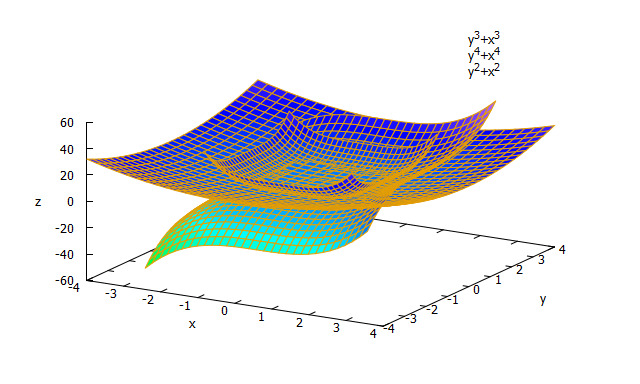
\includegraphics[width=0.75\textwidth]{Pl_explicit_plot3d.png}
	\caption{Multiple 3D explicit plot with different x- and y-ranges for each surface.}
	\label{Pl-Fig7}
\end{SCfigure}

\paragraph{Parametric plot} \mbox{}

\lz A single 3D parametric plot displays a surface generated in parallel by three different expressions (for the x-, y- and z-coordinates) as functions of two common parameters. The names and the ranges of these parameters don't necessarily have anything to do with the names and ranges of the x-, y- and z-coordinates. A multiple parametric plot displays multiple such surfaces. The complete syntax for a single parametric plot is

\lz \tcr{\emph{plot3d ([$ expr_x, \, expr_y, \, expr_z $], [$ p\_name_1, min_1, max_1 $],[$ p\_name_2, min_2, max_2 $] $ \glangle, options \grangle $)}}.

\lz This creates a surface in the three-dimensional space $ expr_x \times expr_y \times expr_z $ in terms of the two common parameters \emph{$ p\_name_1 $} and \emph{$ p\_name_2 $}. 

\lz Neither \emph{x\_range} nor \emph{y\_range} nor \emph{z\_range} have to be present (in the options section). When they are, their names have to be x, y, and z, and they will specify the ranges to be displayed for the two horizontal and the vertical axes. When they are not present, ranges will be set according to the minimum and maximum values of the coordinates of the plot points.

\lz \begin{lstlisting}
<@\tcr{(\%i1)}@   plot3d([t+u,t-u,t*u],[t,0,2],[u,0,2]);
\end{lstlisting}
\vspace{-2mm} 

\begin{SCfigure}[0.33][h]
	\centering
	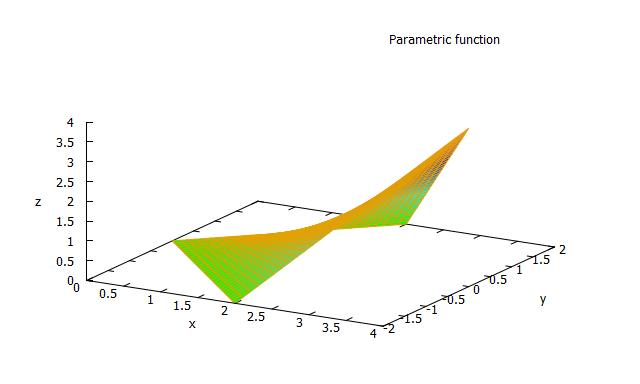
\includegraphics[width=0.75\textwidth]{Pl_parametric_plot3d.png}
	\caption{Single 3D parametric plot.}
	\label{Pl-Fig8}
\end{SCfigure}

\subsubsection{Coordinate transformations for 3D}\label{Pl4}

\lz \emph{plot3d} not only supports standard coordinate transformations from cylindrical or spherical to cartesian coordinates, but in addition lets the user define and apply his own special coordinate transformation functions. This not only allows for giving the expressions to be plotted in cylindrical or spherical coordinates, but in any type of coordinates the user wants.

\paragraph{Standard coordinate transformations} \mbox{}

\lz Standard coordinate transformations predefined for \emph{plot3d} are 

- cylindrical to cartesian (\emph{polar\_to\_xy}), and

- spherical to cartesian (\emph{spherical\_to\_xyz}).

\lz Note that \emph{polar\_to\_xy} cannot be used with plot2d, it is only a 3D feature, and it should have better been called \emph{cylindrical\_to\_xyz}. In the next section we will define our own coordinate transformation carrying precisely this name.

\lz A coordinate transformation is invoked in a \emph{plot3d} with option \emph{transform\_xy}, see section \ref{Pl3}:

\lz \begin{lstlisting}
<@\tcr{(\%i1)}@   plot3d ( 5, [theta, 0, %pi], [phi, 0, 2*%pi], same_xyz,
[transform_xy, spherical_to_xyz]);
\end{lstlisting}
\vspace{-2mm} 

\begin{SCfigure}[0.33][h]
	\centering
	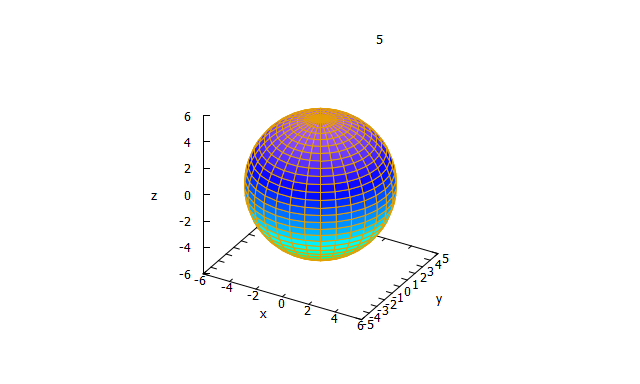
\includegraphics[width=0.75\textwidth]{Pl_explicit_plot3d_spherical.png}
	\caption{3D explicit plot in spherical coordinates.}
	\label{Pl-Fig9}
\end{SCfigure}

\paragraph{User-defined coordinate transformations} \mbox{}

\lz \hyt{make-transform}{\tcr{\emph{make\_transform ([$ cname_1,cname_2,cname_3 $],[$ \, expr_x, \, expr_y, \, expr_z \, $])}}} \hfill \tcr{[function]}\index{make\_transform}

\lz Returns a function suitable to be used in the option \emph{transform\_xy} of \emph{plot3d}. \\
$ cname_1, cname_2, cname_3 $ specify the names of the three new coordinates, and $ \, expr_x, \, expr_y, \, expr_z \, $ their functional expressions to build the cartesian x-, y- and z-coordinates.

\lz As an example, we shall define a coordinate transformation called \emph{cylindrical\_to\_xyz} which is in fact identical to the preconfigured one \emph{polar\_to\_xy}

\lz \begin{lstlisting}
<@\tcr{(\%i1)}@   cylindrical_to_xyz: make_transform([r,phi,z], r*cos(phi), r*sin(phi),z)$
<@\tcr{(\%i2)}@   plot3d (-r, [r, 0, 3], [phi, 0, 2*%pi], [transform_xy, cylindrical_to_xyz]);
\end{lstlisting}
\vspace{-2mm} 

\begin{SCfigure}[0.33][h]
	\centering
	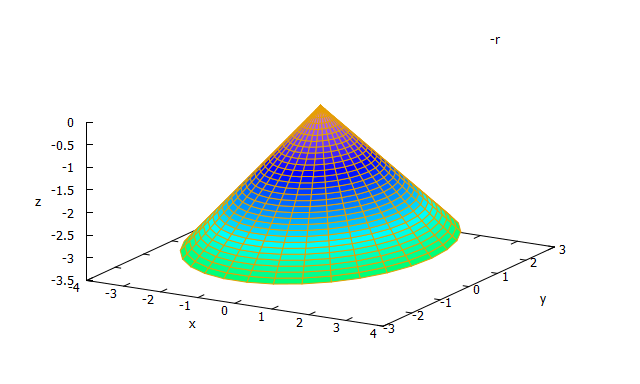
\includegraphics[width=0.75\textwidth]{Pl_explicit_plot3d_cylindrical.png}
	\caption{3D explicit plot in cylindrical coordinates.}
	\label{Pl-Fig10}
\end{SCfigure}

\subsubsection{Options for 3D}\label{Pl3}

\lzz \hyt{plot-same-xyz}{\tcr{\emph{[same\_xyz, true \gbar $ $ false]}}} \qquad \tcr{default: \emph{false}} \hfill \tcr{[plot option]}\index{plot!same\_xyz}

\lz If \emph{true}, the scales of all three axes will be the same.

\lzz \hyt{plot-transform-xy}{\tcr{\emph{[transform\_xy, false \gbar $ $ ct\_name]}}} \qquad \tcr{default: \emph{false}} \hfill \tcr{[plot option]}\index{plot!transform\_xy}

\lz This is a 3D option only. It allows for coodinate transformations within \emph{plot3d}. \emph{ct\_name} is the name of either a predefined coordinate transformation (\emph{polar\_to\_xy} or \emph{spherical\_to\_xyz}), or one defined by the user with \emph{make\_transform}. See section \ref{Pl4} for details.

\section{Draw}

\subsection{Introduction}

This package is a Maxima interface to GNUplot. It allows for significantly more functionality compared to Maxima's propriatory \emph{plot} package, but at the price of a far more complicated syntax.

\lz This package was written and is being maintained by Mario Rodriguez Riotorto. Ample examples can be found in ...

\subsection{General structure}

The \emph{draw} package has to be loaded explicitly by the user with \emph{load(draw)} prior to using it.

\lz \hyt{draw}{\tcr{\emph{draw ($ \dots, \gpal gr2d \gbar gr3d \gpar, \dots \glangle,options \grangle $)}}} \hfill \tcr{[function]}\index{draw}

\lz This main function of the package plots a column of \emph{scenes}, \index{scene} each of them being a picture, a graphical diagram, a plot in either 2D or 3D. Each scene is evoked by an appearance of a scene constructor, either \hyl{gr2d}{\emph{gr2d}}  or \hyl{gr3d}{\emph{gr3d}}, which can be combined in any order and number. General options for all scenes may follow. Each scene can contain multiple graphical objects, e.g. plots. 

\subsubsection{Using options}

\paragraph{General syntax} \mbox{}

\lz The general syntax for options is

\lz \tcr{option\_name = [$ value_1,\dots,value_n $]}.

\lz Global options may appear anywhere in \emph{draw}, \emph{gr2d} or \emph{gr3d}, \emph{draw2d} or \emph{draw3d}, their position does not matter.

\paragraph{Setting defaults for multiple scenes} \mbox{}

\lz \hyt{set\_draw\_defaults}{\tcr{\emph{set\_draw\_defaults ($ opt_1,\dots,opt_m $)}}} \hfill \tcr{[function]}\index{set\_draw\_defaults} \\
\hyt{set\_draw\_defaults}{\tcr{\emph{set\_draw\_defaults ()}}}

\lz The first line sets up user defaults for options to be used for all subsequent scenes. The second line removes all existing user defaults for the subsequent scenes.

\paragraph{Predefined personal sets of options} \mbox{}

\lz In \emph{maxima-init.mac} I have predefined lists of personal default options: \emph{my\_general\_options}, \emph{my\_2d\_options} and \emph{my\_3d\_options}. They can be incorporated as needed in any scene by simply including the respective symbols as global options. 

\lz \begin{lstlisting}
<@\tcr{(\%i1)}@   draw3d(implicit(x^2+y^2=z^2,x,-1,1,y,-1,1,z,-1,1),my_general_options,my_3d_options);
\end{lstlisting}

\lz Alternatively, they can be permanently assigned by \emph{set\_draw\_defaults}. This assignment is not yet done in \emph{maxima-init.mac}, because it depends on the dimension of the plot to be created.

\lz \begin{lstlisting}
<@\tcr{(\%i1)}@   apply(set_draw_defaults,my_general_options);
<@\tcr{(\%i2)}@   draw3d(implicit(x^2+y^2=z^2,x,-1,1,y,-1,1,z,-1,1,my_3d_options));
\end{lstlisting}

\lz Or in case two lists shall be combined:

\lz \begin{lstlisting}
<@\tcr{(\%i1)}@   apply(set_draw_defaults,append(my_general_options,my_3d_options));
<@\tcr{(\%i2)}@   draw3d(implicit(x^2+y^2=z^2,x,-1,1,y,-1,1,z,-1,1));
\end{lstlisting}

\paragraph{User\_preamble} \mbox{}

\lz This option allows to specify certain gnuplot settings which cannot be incorporated with the usual syntax for options.

\lz \tcr{user\_preamble = "$ set \; opt_1; \dots;set \; opt_n $"}

\lz Options are specified by using gnuplot's \emph{set} command followed by the option and possible values. Options are separated by a semicolon.

\lz \begin{lstlisting}
user_preamble = "set raxis; set grid polar; set size 1.1,1.1"
\end{lstlisting}

\subparagraph{Predefined personal user\_preambles} \mbox{}

\lz In \emph{maxima-init.mac} I have a predefined list of options for the user\_preamble in \emph{my\_user\_preamble} which can be easily incorporated into a scene.

\lz \begin{lstlisting}
<@\tcr{(\%i1)}@   draw2d(explicit(x,x,0,1),user_preamble=my_user_preamble);
\end{lstlisting}

\lz The user preamble of a specific scene can contain other options as well.

\lz \begin{lstlisting}
<@\tcr{(\%i1)}@   draw2d(polar(1,theta,0,2*%pi),user_preamble=append(my_user_preamble,["set raxis","set grid polar"]);
\end{lstlisting}

\subsection{2D}

\lz \hyt{gr2d}{\tcr{\emph{gr2d ($ \glangle opt_1,\dots,opt_m, \grangle \, graph\_obj_1,\dots,graph\_obj_n $)}}} \hfill \tcr{[scene constructur]}\index{gr2d}

\lz This is the constructor for a single 2D scene to be used as an argument to function \emph{draw}. Multiple graphical objects $ gobj_1,\dots,gobj_n $ can be plotted within the scene under global options $ opt_1,\dots,opt_m $.

\lzz \hyt{draw2d}{\tcr{\emph{draw2d ($ \glangle opt_1,\dots,opt_m, \grangle \, graph\_obj_1,\dots,graph\_obj_n $)}}} \hfill \tcr{[function]}\index{draw2d}

\hyt{wxdraw2d}{\tcr{\emph{wxdraw2d (...)}}} \hfill \tcr{[function]}\index{wxdraw2d}

\lz These two functions, see this chapter's introduction for their difference, are a shortcut for \emph{\hyl{draw}{draw}(gr2d($ \glangle opt_1,\dots,opt_m, \grangle \, graph\_obj_1,\dots,graph\_obj_n $))}.

\subsubsection{Explicit plot}

\lz \hyt{gobj-explicit}{\tcr{\emph{explicit (f, x, min, max)}}}\hfill \tcr{[graphical object]}\index{explicit!draw object!2D}

\lz A graphical object of this type plots function f, given in explicit form, with the independent variable x in the range from x=min to x=max. 

\paragraph{Piecewise defined function} \mbox{}

\lz In combination with the global options \emph{xrange} and \emph{yrange} it is possible to plot a piecewise defined function.

\lz \begin{lstlisting}
<@\tcr{(\%i1)}@   draw2d(explicit(0.5,x,0,1),explicit(1,x,1,2),explicit(1.5,x,2,3),xrange=[0,3],yrange=[0,2]);
\end{lstlisting}

\begin{SCfigure}[1.0][h]
	\centering
	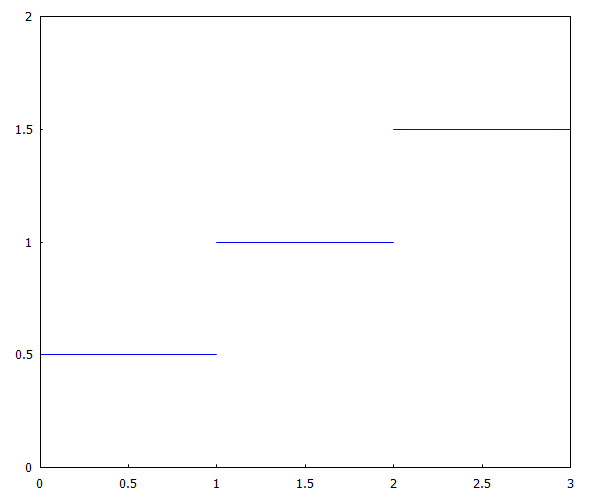
\includegraphics[width=0.5\textwidth]{Pl_draw_piecewise.png}
	\caption{Plotting a piecewise defined function with draw.}
	\label{Pl-Fig11}
\end{SCfigure}

\subsubsection{Implicit plot}

\lz \hyt{gobj-implicit}{\tcr{\emph{explicit (f, x, min, max)}}}\hfill \tcr{[graphical object]}\index{implicit!draw object!2D}

\lz A graphical object of this type plots function f, given in implicit form, with dependent variable x in the range from x=min to x=max. Note that in combination with the global option \emph{xrange} it is possible to plot a piecewise defined function.

\subsubsection{Polar plot}

\lz \hyt{gobj-polar}{\tcr{\emph{polar (radius, ang, $ ang_{min}, ang_{max} $)}}}\hfill \tcr{[graphical object]}\index{polar!draw object}

\lz Plots the radius as a function of the angle in the given range. This object can be plotted with an underlying polar grid, see thread in maxima-discuss from March 2019.

\lz \begin{lstlisting}
<@\tcr{(\%i1)}@   draw2d(polar(1-(theta/(2*%pi)),theta,0,2*%pi), xrange=[-1,1], yrange=[-1,1], proportional_axes = xy, user_preamble="set raxis; set grid polar");
\end{lstlisting}

\begin{SCfigure}[0.6][h]
	\centering
	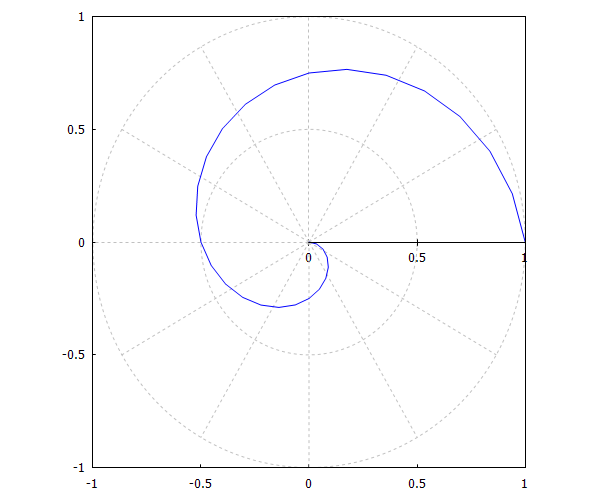
\includegraphics[width=0.6\textwidth]{Pl_draw_polar_grid.png}
	\caption{Plotting a function in polar coordinates and with an underlying polar grid with draw.}
	\label{Pl-Fig12}
\end{SCfigure}

\lz Underlying cartesian and polar grids can be combined, too.

\lz \begin{lstlisting}
<@\tcr{(\%i1)}@   draw2d(polar(1-(theta/(2*%pi)),theta,0,2*%pi), xrange=[-1,1], yrange=[-1,1], proportional_axes = xy, grid=true, user_preamble="set raxis; set grid polar");
\end{lstlisting}

\begin{SCfigure}[0.6][h]
	\centering
	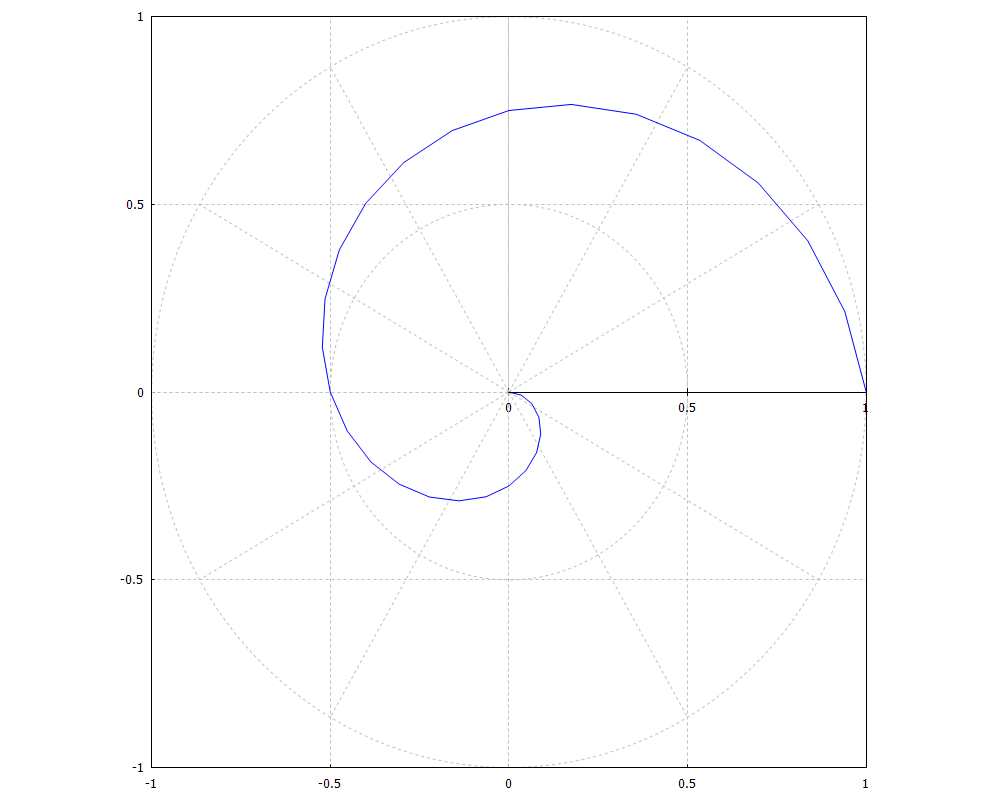
\includegraphics[width=0.6\textwidth]{Pl_draw_polar_double_grid.png}
	\caption{Plotting a function in polar coordinates and with aunderlying cartesian and polar grids with draw.}
	\label{Pl-Fig13}
\end{SCfigure}

\subsection{3D}

\lz \hyt{gr3d}{\tcr{\emph{gr3d ($ \glangle opt_1,\dots,opt_m, \grangle \, graph\_obj_1,\dots,graph\_obj_n $)}}} \hfill \tcr{[scene constructur]}\index{gr3d}

\lz This is the constructor for a single 3D scene to be used as an argument to function \emph{draw}. Multiple graphical objects $ gobj_1,\dots,gobj_n $ can be plotted within the scene under global options $ opt_1,\dots,opt_m $.

\lzz \hyt{draw3d}{\tcr{\emph{draw3d ($ \glangle opt_1,\dots,opt_m, \grangle \, graph\_obj_1,\dots,graph\_obj_n $)}}} \hfill \tcr{[function]}\index{draw3d}

\hyt{wxdraw3d}{\tcr{\emph{wxdraw3d(...)}}} \hfill \tcr{[function]}\index{wxdraw3d}

\lz These two functions, see this chapter's introduction for their difference, are a shortcut for \emph{\hyl{draw}{draw}(gr3d($ \glangle opt_1,\dots,opt_m, \grangle \, gobj_1,\dots,gobj_n $))}.

\subsubsection{Explicit plot}

\lz \hyt{gobj-explicit}{\tcr{\emph{explicit ($ f, x, x_{min}, x_{max}, \, y, y_{min}, y_{max} $)}}}\hfill \tcr{[graphical object]}\index{explicit!draw objects!3D}

\lz A graphical object of this type plots function f, given in explicit form, with the independent variables x and y in the given ranges. 

\lz Just like in the 2D case, in combination with the global options \emph{xrange}, \emph{yrange} and \emph{zrange} it is possible to plot a piecewise defined function.

\subsubsection{Implicit plot}

\lz \hyt{gobj-implicit}{\tcr{\emph{implicit ($ f, x, x_{min}, x_{max}, \, y, y_{min}, y_{max}, \, z, z_{min}, z_{max} $)}}}\hfill \tcr{[graphical object]}\index{implicit!draw objects!3D}

\lz A graphical object of this type plots function f, given in implicit form, with dependent variable x in the range from x=min to x=max. Note that in combination with the global option \emph{xrange} it is possible to plot a piecewise defined function.

\subsection{List of available options}

\lz \hyt{proportional-axes}{\tcr{\emph{proportional\_axes=$ \gpal xy \gbar xyz \gpar $}}} \qquad \tcr{default: \emph{none}} \hfill \tcr{[plot option]}\index{proportional\_axes!draw option}

\lz Displays with the specified axes proportional to their relative lengths. The value \emph{xy} can be used for 3D, too.

\lzz \hyt{draw-xrange}{\tcr{\emph{xrange=[min,max]
}}} \qquad \tcr{default: \emph{auto}} \hfill \tcr{[plot option]}\index{xrange!draw option!2D}

\lz Specifies the range of the x-axis for this scene. If this option is missing, the minimal range used by the graphical objects will be shown in the scene.

\lzz \hyt{draw-yrange}{\tcr{\emph{yrange=[min,max]}}} \qquad \tcr{default: \emph{auto}} \hfill \tcr{[plot option]}\index{draw option!2D!yrange}

\lz Specifies the range of the y-axis for this scene. If this option is missing, the minimal range used by the graphical objects will be shown in the scene. 

\end{document}